\section{Исследование наблюдаемости}

Рассмотрим систему: 
\begin{equation}
    \begin{cases}
        \dot{x} = Ax \\
        y = Cx,
    \end{cases}
\end{equation}
где 
\begin{equation}
    \begin{array}{cc}
        A = \begin{bmatrix}
            -10 & -7 & -18 \\
            -3 & -4 & -8 \\
            8 & 2 & 11
        \end{bmatrix}, &
        C = \begin{bmatrix}
            2 & -3 & 1
        \end{bmatrix}
    \end{array}
\end{equation}

\subsection{Наблюдаемость системы}

\subsubsection{Матрица наблюдаемости}
Найдем матрицу наблюдаемости $W = [C, CA, CA^2]^T$: 
\begin{equation}
    W = \begin{bmatrix}
        2  & -3  & 1 \\ 
        -3  & 0  & -1 \\ 
        22  & 19  & 43 \\ 
    \end{bmatrix}
\end{equation}
Определим ранг матрицы наблюдаемости:
\begin{equation}
    \text{rank}(W) = 3
\end{equation}
Таким образом, система является полностью наблюдаемой.

\subsubsection{Наблюдаемость собственных значений}

Найдем спектр матрицы $A$:
\begin{equation}
    \sigma(A) = \{1, -2-5j, -2+5j\}
\end{equation}
Для каждого собственного значения найдем матрицу Хаутуса $H_i = [A - \lambda_i, C]^T$:
\begin{enumerate}
    \item $\lambda_1 = 1$: $H_1 = \begin{bmatrix}
        -11 & -7 & -18 \\
        -3 & -5 & -8 \\
        8 & 2 & 10 \\
        2 & -3 & 1
    \end{bmatrix}$, $\text{rank}(H_1) = 3$, собственное значение наблюдаемо.
    \item $\lambda_2 = -2-5j$: $H_2 = \begin{bmatrix}
        -8+5j & -7 & -18 \\
        -3 & -2+5j & -8 \\
        8 & 2 & 13+5j \\
        2 & -3 & 1
    \end{bmatrix}$, $\text{rank}(H_2) = 3$, собственное значение наблюдаемо.
    \item $\lambda_3 = -2+5j$: $H_3 = \begin{bmatrix}
        -8-5j & -7 & -18 \\
        -3 & -2-5j & -8 \\
        8 & 2 & 13-5j \\
        2 & -3 & 1
    \end{bmatrix}$, $\text{rank}(H_3) = 3$, собственное значение наблюдаемо.
\end{enumerate}
Все собственные значения наблюдаемы, что сходится с результатом, полученным при анализе матрицы наблюдаемости.

\subsubsection{Диагональная форма системы}
Найдем диагональную форму системы:
\begin{equation}
    \begin{cases}
        \dot{\hat{x}} = P^{-1}AP\hat{x}\\
        y = CP\hat{x},
    \end{cases}
\end{equation}
где $P$ -- матрица собственных векторов матрицы $A$. Найдем собственные векторы матрицы $A$:
\begin{equation}
    \begin{array}{ccc}
        v_1 = \begin{bmatrix}
            -1 \\
            -1 \\
            1
        \end{bmatrix}, &
        v_2 = \begin{bmatrix}
            -1.5-0.5j \\
            -1.5-0.5j \\
            1
        \end{bmatrix}, &
        v_2 = \begin{bmatrix}
            -1.5+0.5j \\
            -1.5+0.5j \\
            1
        \end{bmatrix}
    \end{array}
\end{equation}
Тогда матрица $P$:
\begin{equation}
    P = \begin{bmatrix}
        -1 & -1.5-0.5j & -1.5+0.5j \\
        -1 & -1.5-0.5j & -1.5+0.5j \\
        1 & 1 & 1
    \end{bmatrix}
\end{equation}
Система преобразуется к виду: 
\begin{equation}
    \begin{cases}
        \dot{\hat{x}} = \begin{bmatrix}
            1 & 0 & 0 \\
            0 & -2-5j & 0 \\
            0 & 0 & -2+5j
        \end{bmatrix} \hat{x} \\ 
        y = \begin{bmatrix}
            2 & -0.5+0.5j & -0.5-0.5j
        \end{bmatrix} \hat{x}
    \end{cases}
\end{equation}
Так как все элементы матрицы $CP$ не равны нулю, система является полностью наблюдаемой. 

\subsection{Грамиан наблюдаемости}
Найдем грамиан наблюдаемости $Q(t_1)$:
\begin{equation}
    Q(t_1) = \int_0^{t_1} e^{A^Tt}C^TCe^{At}dt
\end{equation}
Вычислим грамиан наблюдаемости для $t_1 = 3$:
\begin{equation}
    Q(3) = \begin{bmatrix}
        804.17  & -804.51  & 804.12 \\ 
        -804.51  & 805.18  & -804.28 \\ 
        804.12  & -804.28  & 804.22 \\ 
        \end{bmatrix}
\end{equation}
Найдем собственные числа грамиана наблюдаемости:
\begin{equation}
    \sigma(Q(3)) = \{0.013, 0.42, 2413.13\}
\end{equation}
Все собственные числа грамиана наблюдаемости положительны, что говорит о том, что система является наблюдаемой.

\subsection{Наблюдение системы}
Будем считать, что выход системы соответствует функции $y(t)$:
\begin{equation}
    y(t) = e^{-2t} \cos(5t) -2e^{-2t} \sin(5t) 
\end{equation}
Найдем начальные условия $x(0)$ такие, чтобы выход системы совпадал с функцией $y(t)$:
\begin{equation}
    x(0) = Q(t_1)^{-1} \int_0^{t_1} e^{A^Tt}C^Ty(t)dt
\end{equation}
Получаем вектор начальных условий:
\begin{equation}
    x(0) = \begin{bmatrix}
        3 & 1 & -2
    \end{bmatrix}^T
\end{equation}

Проведем моделирование системы с начальными условиями $x(0)$ и входом $u(t) = 0$: 
\begin{figure}
    \centering
    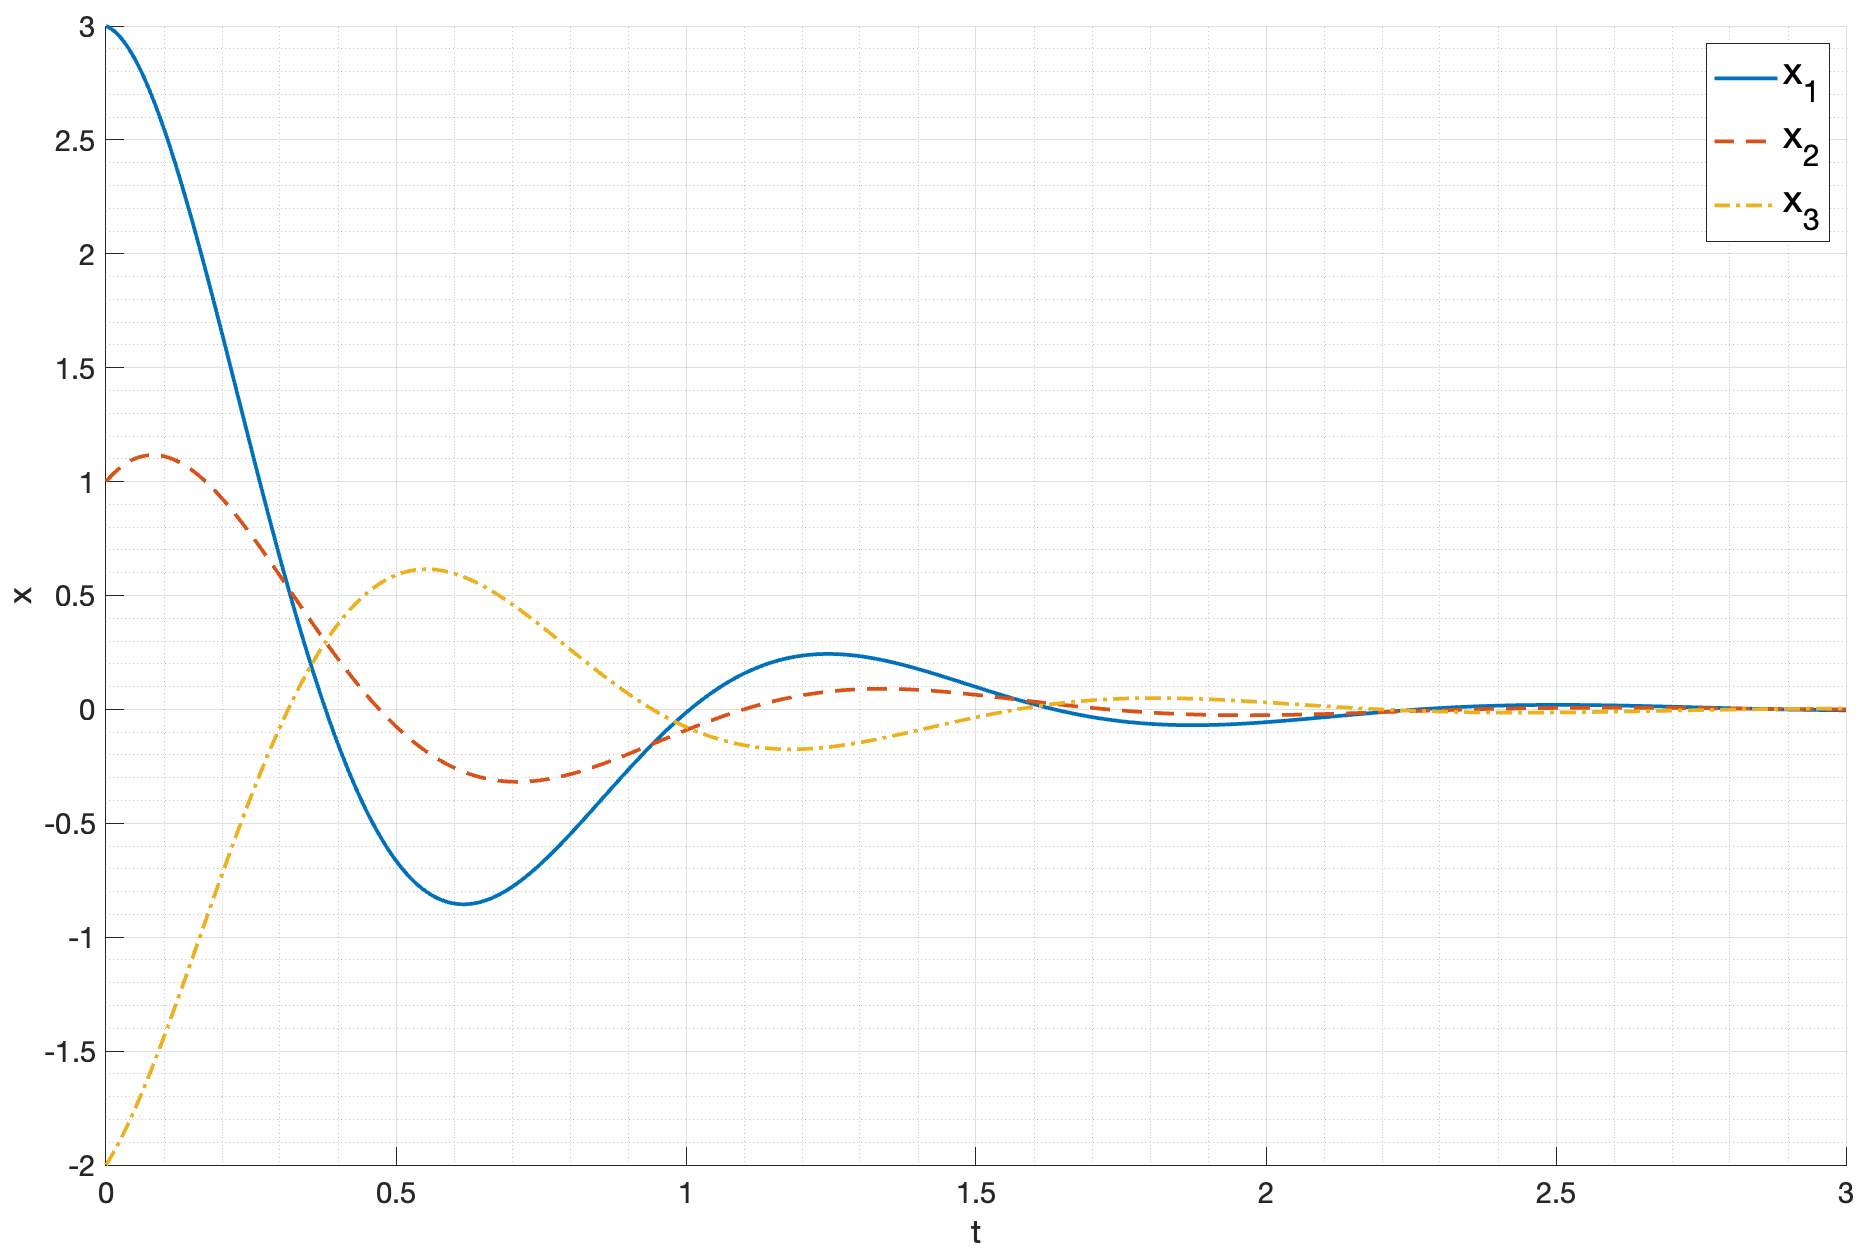
\includegraphics[width=\textwidth]{media/plots/task3_states.png}
    \caption{Состояния системы}
    \label{fig:task3_states}
\end{figure}
На рисунке \ref{fig:task3_states} изображены состояния системы.
\begin{figure}
    \centering
    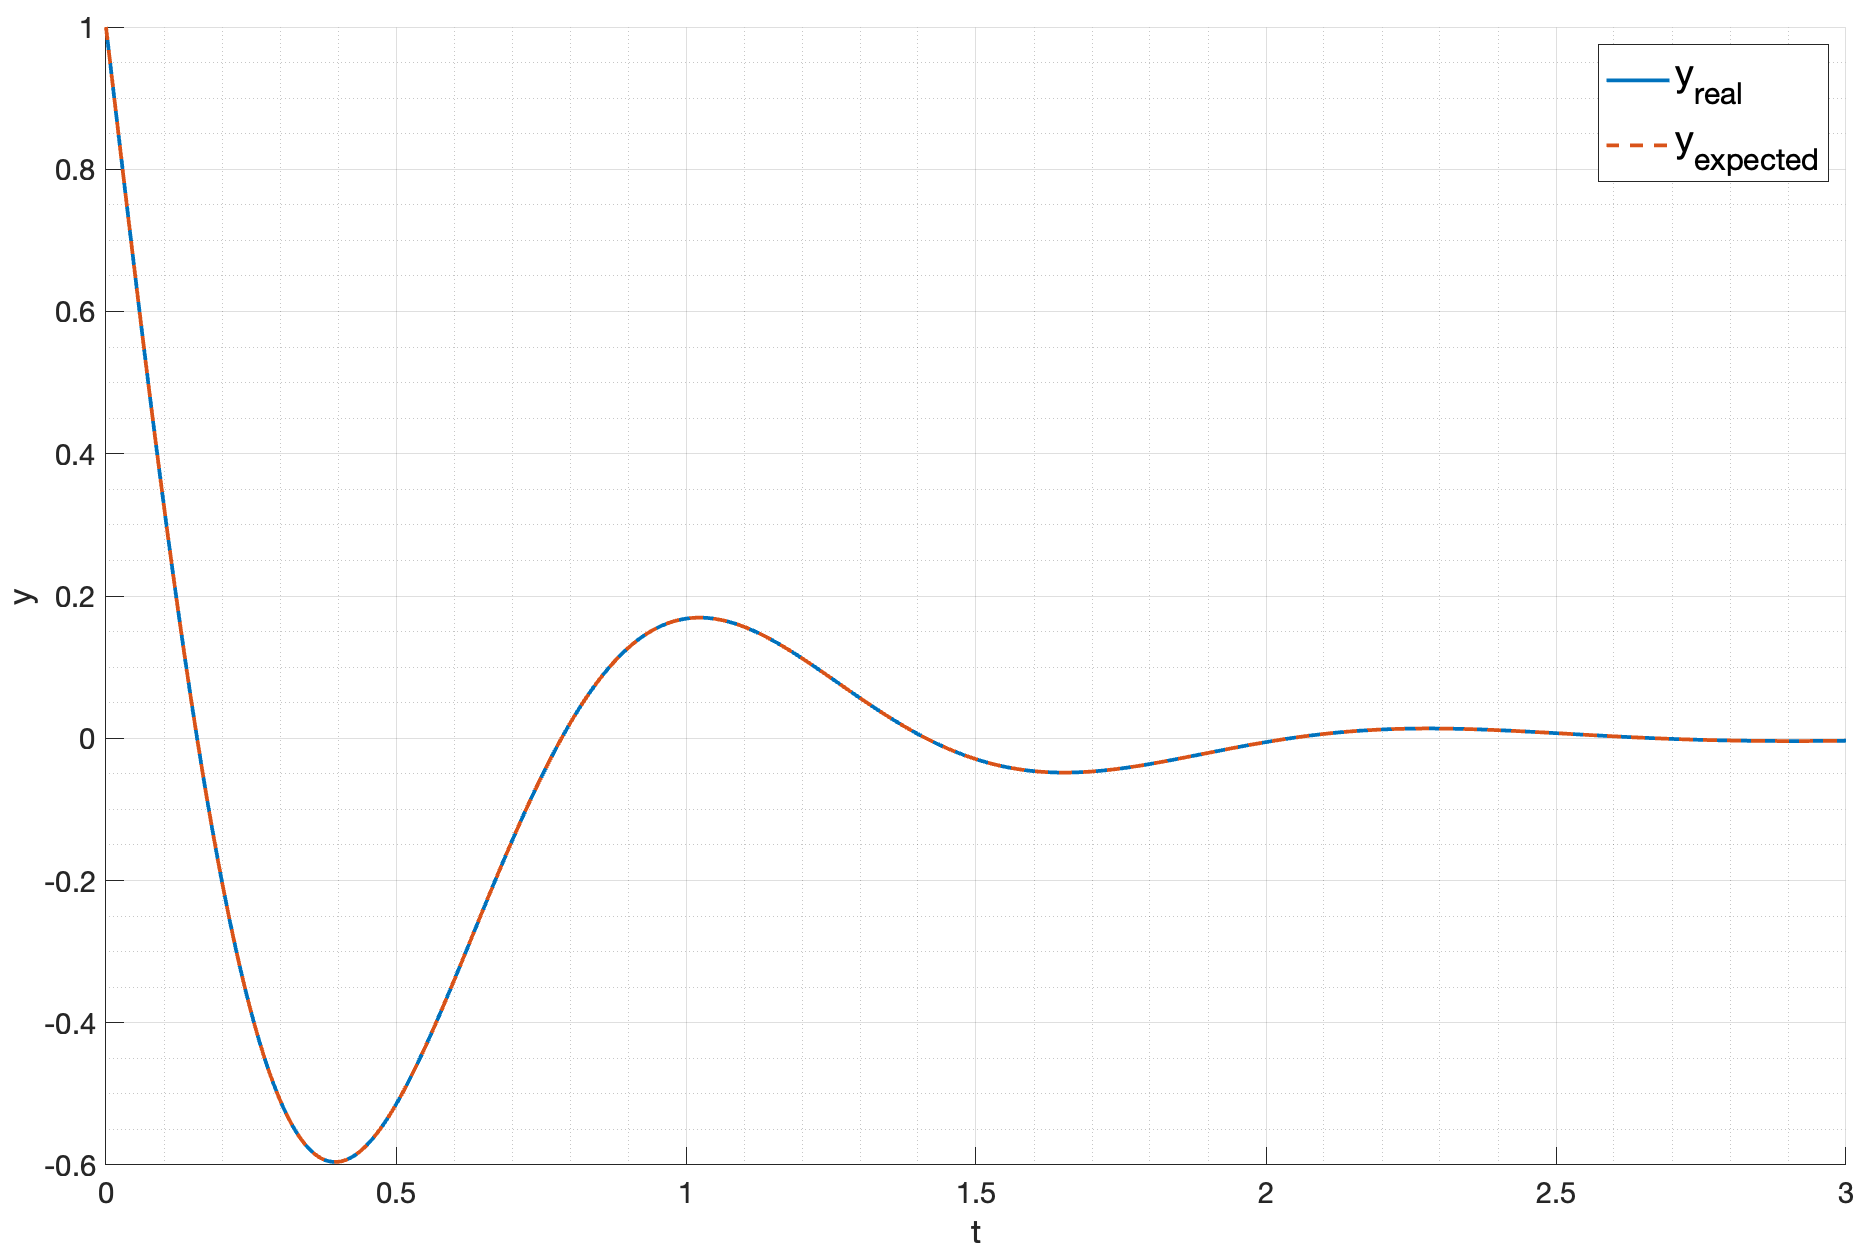
\includegraphics[width=\textwidth]{media/plots/task3_output.png}
    \caption{Выход системы}
    \label{fig:task3_output}
\end{figure}
На рисунке \ref{fig:task3_output} изображен выход системы. Видно, что выход системы совпадает с функцией $y(t)$.
\begin{figure}
    \centering
    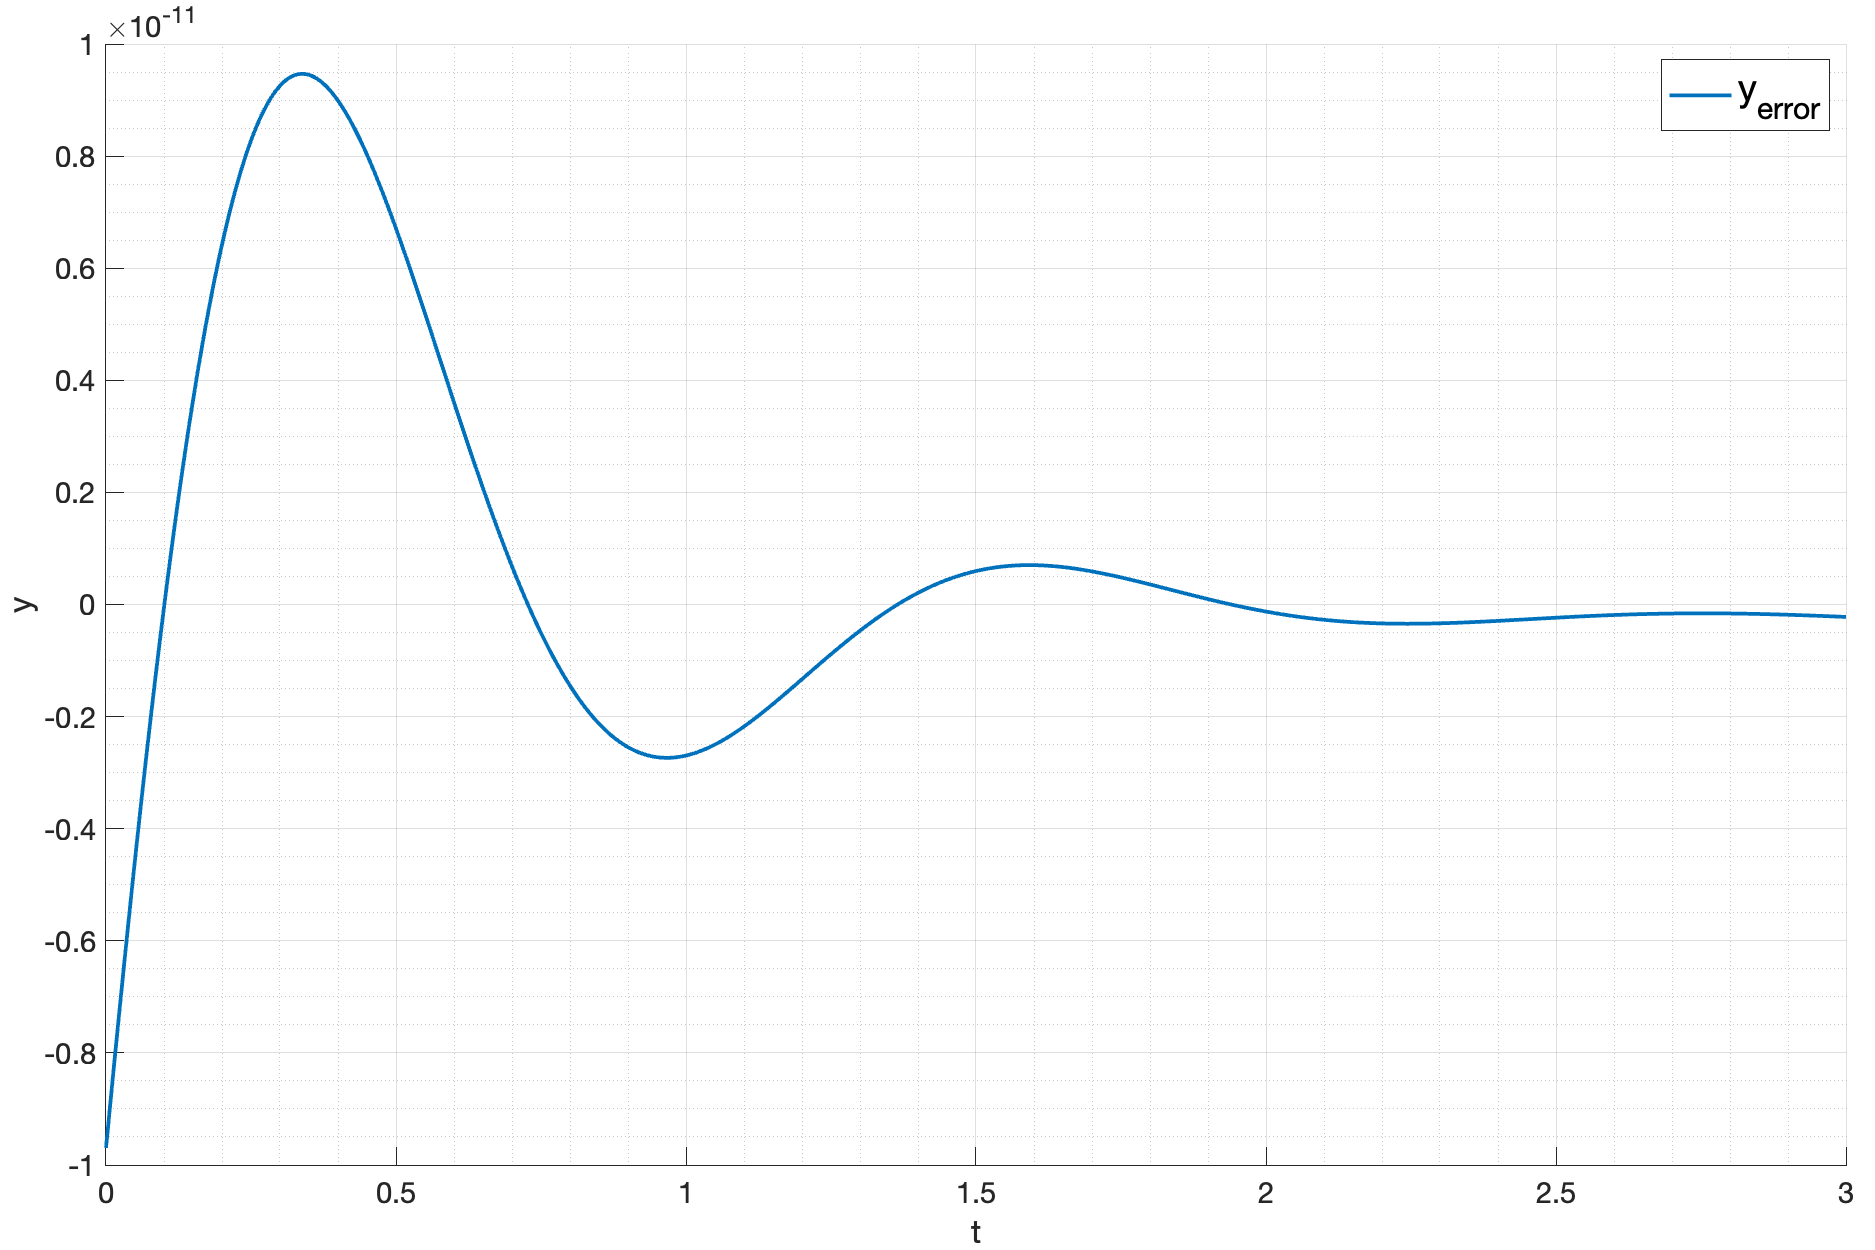
\includegraphics[width=\textwidth]{media/plots/task3_error.png}
    \caption{Ошибка наблюдения}
    \label{fig:task3_estimation}
\end{figure}
На рисунке \ref{fig:task3_estimation} изображена ошибка наблюдения. Видно, что ошибка наблюдения стремится к нулю
и не превышает $10^{-11}$.

\FloatBarrier
\subsection{Вывод}
При исследовании системы, рассматриваемой в этом задании, удалось показать,
что она является полностью наблюдаемой. Это было продемонстрировано с помощью
матрицы наблюдаемости, через наблюдаемость собственных значений и диагональную
форму системы. Также был найден грамиан наблюдаемости и проверены его собственные
числа. Проведено моделирование системы с начальными условиями, при которых выход
системы совпадает с заданной функцией. Результаты моделирования показали, что
система наблюдаема и наблюдение работает корректно.